\section{Proyecto LINCE}

El trabajo que recoge esta memoria se enmarca aquí: en el subsistema de comunicaciones del
ordenador de a bordo (OBC), del que la UPM es responsable dentro del consorcio.

El Proyecto LINCE (Línea de industrialización de cargas de pago y plataformas espaciales) es
una iniciativa estratégica enmarcada en el PERTE Aeroespacial, cuyo propósito es consolidar
la capacidad industrial de España en el segmento de los microsatélites (100--200 kg)
destinados a órbitas bajas (LEO). Liderado por Indra, el consorcio busca desarrollar
plataformas satelitales modulares, fiables y de altas prestaciones, optimizando costes y
plazos mediante procesos de producción en serie. Este ecosistema integra a grandes
empresas, PYMES y centros de investigación, como la Universidad Politécnica de Madrid
(UPM), para habilitar servicios avanzados de telecomunicaciones, vigilancia y observación,
garantizando así la autonomía estratégica de España y Europa en el sector espacial
\cite{indra2026lince}.

\section{MPSoC Zynq UltraScale+ ZCU102}

El OBC del satélite se construye sobre este MPSoC, y la ZCU102 es la plataforma sobre la que se
ha desarrollado y validado este trabajo. Es una tarjeta de evaluación de propósito general de Xilinx (hoy AMD) para el prototipado de
sistemas empotrados sobre el MPSoC (\textit{Multiprocessor System-on-Chip}) Zynq UltraScale+.
Este MPSoC integra en un único encapsulado un sistema de procesamiento con cuatro núcleos ARM
(\textit{Advanced RISC Machines}) y una matriz de lógica programable, unidos por buses internos de
alto rendimiento. La arquitectura
separa el sistema en dos dominios complementarios: el Sistema de Procesamiento (PS,
\textit{Processing System}) y la lógica programable (PL, \textit{Programmable Logic}).

El \textbf{PS} es el dominio del software. Son núcleos ARM de arquitectura fija que ejecutan
instrucciones de forma secuencial, igual que cualquier microprocesador clásico. Sobre ellos
corren el sistema operativo, la gestión de la memoria DDR (\textit{Double Data Rate}) y las
rutinas de control de alto nivel.

La \textbf{PL} es el dominio del hardware a medida: una matriz reconfigurable tipo FPGA
(\textit{Field Programmable Gate Array}) que no ejecuta un programa, sino que se configura físicamente. Con un
lenguaje de descripción de hardware como VHDL (\textit{Very High Speed Integrated Circuit
Hardware Description Language}) se interconectan los recursos del silicio (tablas de búsqueda,
biestables, memoria BRAM (\textit{Block RAM}) y bloques DSP (\textit{Digital Signal Processor}))
para formar circuitos digitales concretos.
A cambio de un flujo de diseño más costoso, la PL ofrece determinismo temporal estricto y
paralelismo masivo.

La placa expone dos conectores FMC (\textit{FPGA Mezzanine Card}) HPC (\textit{High Pin Count}), conformes al estándar VITA 57.1
\cite{vita571fmc}. Sobre ellos se montan tarjetas de expansión (\textit{mezzanines}) que llevan
pines digitales y pares diferenciales de la FPGA hacia el exterior, que es la vía para conectar
periféricos físicos a la PL.

La figura~\ref{fig:mpsoc_zynq} recoge el reparto. Conviene fijarse en los puertos AXI entre PS y
PL, porque son el camino que recorren los datos de los catorce enlaces serie y el objeto de la
comparativa del capítulo~4.

\begin{figure}[htbp]
    \centering
    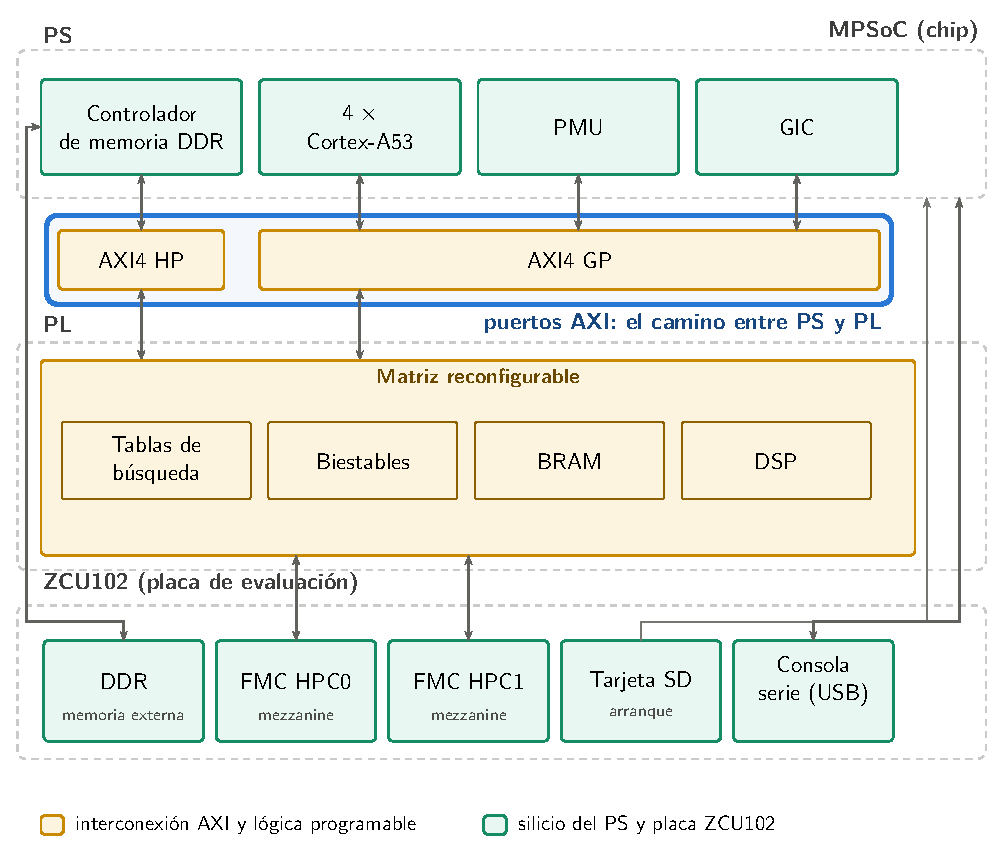
\includegraphics[width=\textwidth]{IMG/Desarrollo/diagrama_mpsoc_zynq.pdf}
    \caption{MPSoC Zynq UltraScale+ y entorno de la ZCU102.}
    \label{fig:mpsoc_zynq}
\end{figure}

\section{Vivado y Vitis (Xilinx): PS y PL}

Estas dos herramientas son las que han producido todo lo desarrollado en este trabajo: el VHDL
que ocupa la PL y el código C que corre en el PS. Xilinx distribuye dos entornos para el desarrollo sobre el Zynq UltraScale+: Vivado para la PL y
Vitis para el PS.

\subsection{Vivado Design Suite}

En Vivado se diseñó e implementó toda la lógica que ocupa la PL, desde el transceptor serie
hasta los puentes de transporte. Vivado es el entorno de diseño, síntesis e implementación de la lógica de la PL. Admite
descripción en HDL (\textit{Hardware Description Language}) y diseño por bloques (\textit{Block
Design}), donde los periféricos de diseño propio se conectan al PS mediante el bus AXI
(\textit{Advanced eXtensible Interface}). El fichero de
restricciones (.xdc) asocia las señales del diseño a los pines físicos del encapsulado. El flujo
termina con dos salidas: el \textit{bitstream} que configura la FPGA y un fichero .xsa que
describe la arquitectura hardware para las herramientas de software.

Los periféricos de diseño propio se integran con el procesador dentro de Vivado, que además
dirige sus señales hasta los conectores FMC.

\subsection{Vitis Unified Software Platform}

En Vitis se construyó el software que corre en el PS, tanto el driver como las aplicaciones de
prueba. Vitis es el IDE para el software del PS. Toma el fichero .xsa de Vivado y genera el paquete de
soporte de la placa (BSP, \textit{Board Support Package}): el mapa de memoria y los \textit{drivers}
de bajo nivel con los que el código en C accede a los periféricos de la PL. Aporta además el
compilador cruzado para los núcleos ARM y el empaquetado del binario de arranque (BOOT.BIN), que
reúne el firmware de inicialización (PMUFW, \textit{Power Management Unit Firmware}, y FSBL,
\textit{First Stage Boot Loader}), el \textit{bitstream} y el ejecutable en un
solo fichero cargable desde una tarjeta SD.

Con Vitis se construyen, por tanto, tanto la capa de acceso a los periféricos como la imagen con
la que la placa arranca de forma autónoma.

\section{RTEMS}

RTEMS es el sistema operativo bajo el que se ejecuta el software de vuelo, y por tanto el que
tiene que dar servicio al driver desarrollado aquí. RTEMS (\textit{Real-Time Executive for Multiprocessor Systems}) es un sistema operativo de tiempo
real de código abierto para sistemas empotrados de misión crítica. No usa memoria virtual:
opera en un único espacio de direcciones físico, con un solo proceso y varios hilos. Al no haber
cambios de contexto pesados ni traducción de direcciones, la latencia de respuesta a una
interrupción es baja y acotada.

Es un estándar de facto en la industria aeroespacial (ESA, \textit{European Space Agency}, y NASA
lo emplean en satélites y sondas) por su robustez y su soporte para arquitecturas ARM como la del
Zynq UltraScale+. En
este tipo de plataforma se ejecuta sobre el PS y se encarga de la lógica de control y del acceso
a los registros de los periféricos de la PL. El acceso a un periférico de diseño propio no
cuenta con driver previo en RTEMS: da control total sobre la lógica y sobre cada registro, a
cambio de una curva de aprendizaje y una complejidad de desarrollo mayores que las de un
periférico ya integrado.

\section{Comunicaciones serie}

El OBC de LINCE debe atender enlaces de estos cuatro tipos. Sus características eléctricas y
sus formatos de trama son los que fijan lo que el transceptor tiene que soportar. En arquitecturas satelitales, las comunicaciones serie son el medio habitual de intercambio de
datos entre el ordenador de a bordo (OBC) y sus periféricos: sensores, actuadores y cargas de
pago. Frente al bus paralelo, el enlace serie reduce drásticamente el número de líneas físicas,
y con ello el peso y el volumen del arnés. La señalización diferencial, común a la mayoría de
estos estándares, cancela en el receptor el ruido electromagnético inducido por igual en los dos
hilos.

Los cuatro estándares que se describen a continuación (RS485, RS422, SpaceWire y CAN) cubren ese
papel con topologías y prestaciones distintas.

\subsection{RS485}

Es el estándar que hace posible el bus compartido de siete nodos de la placa de comunicación
serie. El estándar TIA/EIA-485 (RS485) define las características eléctricas de transmisores y
receptores para enlaces serie diferenciales. Su rasgo distintivo es la topología multipunto:
admite hasta 32 transceptores estándar sobre el mismo par de hilos, más si son de carga
fraccional\footnote{Receptores que cargan la línea con una fracción de la unidad estándar, lo que permite superar los 32 nodos.}.

La información viaja como diferencia de tensión entre los hilos A y B, lo que da un alto rechazo
al modo común. Se suele usar en \textit{half-duplex} sobre dos hilos, con transmisión y recepción
compartiendo el medio; esto obliga a controlar por software el sentido del enlace (pines de
\textit{driver enable}) para evitar colisiones. Alcanza unos 1200~m a baja velocidad o hasta
decenas de Mbps en distancias cortas, y necesita resistencias de terminación de $120\,\Omega$ en
los extremos del bus para evitar reflexiones\footnote{Ecos de la señal en un extremo mal adaptado de la línea, que se superponen a los bits siguientes.}~\cite{ti2014rs485,eia485a}.

\subsection{RS422}

Sobre él se montan los dos buses \textit{master/slave} de esa misma placa. El estándar TIA/EIA-422 (RS422) comparte con el RS485 la señalización diferencial, pero no la
topología: está pensado para enlaces punto a punto o \textit{multi-drop}\footnote{Un transmisor y varios receptores sobre el mismo par; los receptores no transmiten por esa línea.}, con un único transmisor
y hasta 10 receptores por par.

Los transceptores RS422 no ceden el control del bus, así que la comunicación bidireccional
continua (\textit{full-duplex}) exige cuatro hilos: un par para transmisión y otro para recepción.
Al separar físicamente los dos sentidos, no hace falta arbitrar el bus por software, lo que
reduce la carga de proceso y hace el enlace idóneo para el envío continuo de telemetría de
sensores~\cite{ti2018rs422,tia422b}.


La figura~\ref{fig:topologia_rs} contrapone las dos topologías. En RS485 los nodos cuelgan del
mismo par y solo uno transmite a la vez, de modo que hace falta la señal \texttt{DE} para cederse
el medio. En RS422 cada par tiene un único transmisor, y por eso el enlace no necesita arbitraje.

\begin{figure}[htbp]
    \centering
    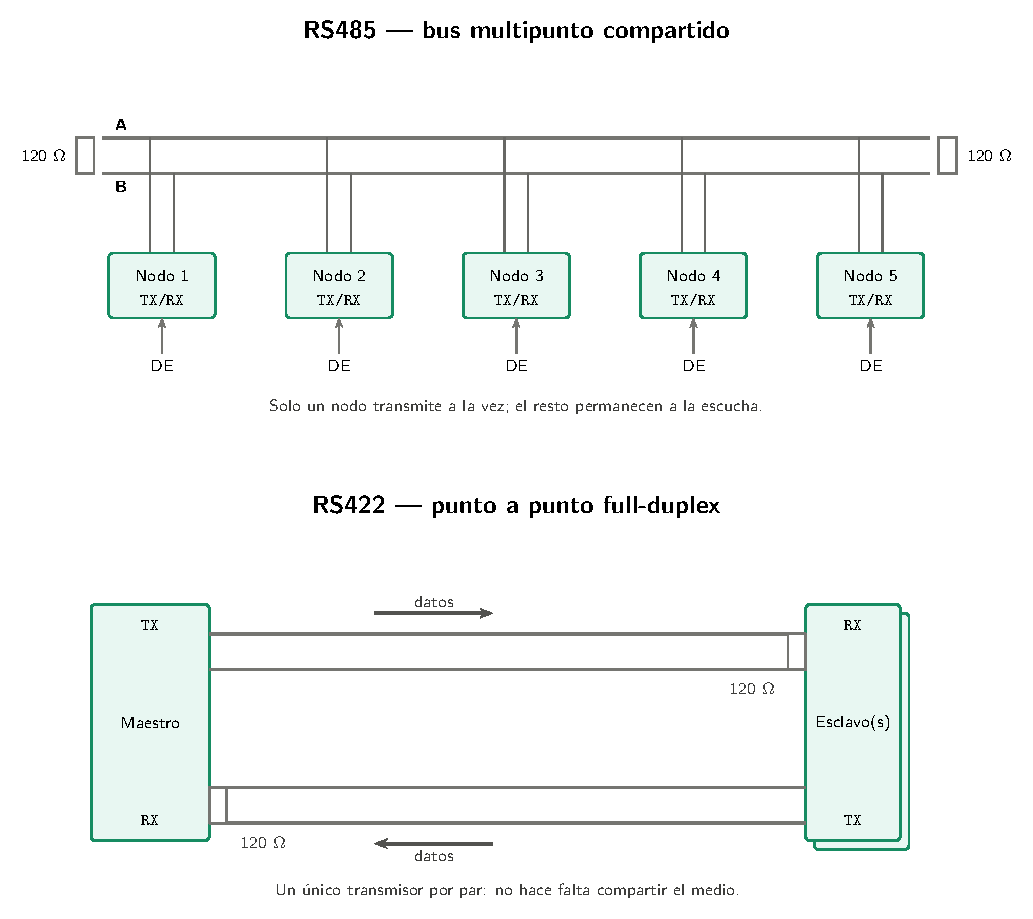
\includegraphics[width=0.92\textwidth]{IMG/Desarrollo/diagrama_topologia_rs.pdf}
    \caption{Topologías RS485 y RS422.}
    \label{fig:topologia_rs}
\end{figure}

\subsection{SpaceWire}

La placa AOCS expone dos enlaces SpaceWire, la única interfaz de las tres placas que quedó sin
validar. SpaceWire es un estándar de red a bordo de alta velocidad coordinado por la ESA, usado para
interconectar nodos de alto rendimiento como memorias masivas, procesadores de instrumento y
enlaces de telemetría.

En el nivel físico usa señalización LVDS\footnote{\textit{Low-Voltage Differential Signaling}: par diferencial de unos 350~mV de excursión, para alta velocidad y bajo consumo.} y una codificación \textit{Data-Strobe}. Enviar el reloj
por un par propio obliga a que ese par y el de datos lleguen alineados dentro de una fracción del
tiempo de bit. A 200~Mbps el tiempo de bit es de 5~ns, de modo que un desfase de pocos
nanosegundos entre ambos pares, acumulado por la diferencia de longitud de las pistas y por la
dispersión del cable, basta para muestrear el bit equivocado.

La codificación \textit{Data-Strobe} evita esa restricción. Los datos viajan por un par y una
señal \textit{strobe} por el otro, con la condición de que en cada bit conmute una sola de las
dos. El reloj se recupera con una XOR entre ambas, y el margen deja de depender del alineamiento
entre pares para depender solo de que ninguno cambie dos veces en el mismo
bit~\cite{ecss50spw,parkes2012spw}. Proporciona enlaces punto a punto \textit{full-duplex}
asíncronos de hasta 400~Mbps. Su pila incluye una capa de red que permite encaminar
paquetes a través de \textit{routers} SpaceWire~\cite{ecss50spw,parkes2012spw}.

\subsection{CAN}

La placa CDHS lleva un bus CAN redundante, y su validación es uno de los resultados del
capítulo~4. El bus CAN (\textit{Controller Area Network}) nació en automoción y se usa como estándar de facto
(\textit{CAN for Aerospace}) en
las redes internas de telemetría y telecomando (TM/TC) de satélites pequeños y comerciales.

Es multipunto y multimaestro, con acceso por escucha de portadora, es decir, cada nodo espera a
que el bus esté en reposo antes de empezar a transmitir, y con arbitraje por prioridad de
mensaje. Los nodos no tienen dirección: cada trama lleva un identificador que fija su contenido y
su prioridad. Si dos nodos transmiten a la vez, la colisión se resuelve bit a bit y sin destruir
datos: gana el identificador de mayor prioridad y el otro nodo reintenta. La capa de enlace añade
detección de errores por hardware (CRC, \textit{bit stuffing}\footnote{Inserción de un bit de polaridad contraria tras cinco bits iguales para que el receptor mantenga el sincronismo.}, comprobación de trama) y
aislamiento automático de nodos defectuosos, de modo que un periférico averiado no bloquea el
bus~\cite{iso118981,esa2015can}.
